\chapter{Research Design}\label{chap:research-design}

The research design is the general plan for conducting a study, ensuring that the research questions are addressed effectively.
According to \textcite{SaundersMark2023}, the research design outlines the overall strategy that integrates the different components of the study in a coherent and logical manner, thus ensuring that the study effectively addresses the research question.
Fig.~\ref{fig:research-onion} illustrates the research onion, which provides a structured approach to the conceptualisation of research design by stripping away various layers, including research philosophy, research approach, methodological choice, strategy, time horizon, and data collection techniques and procedures.
This chapter will briefly discuss each of these layers, providing a comprehensive overview of the chosen research design for this study.

\begin{figure}[htbp]
    \centering
 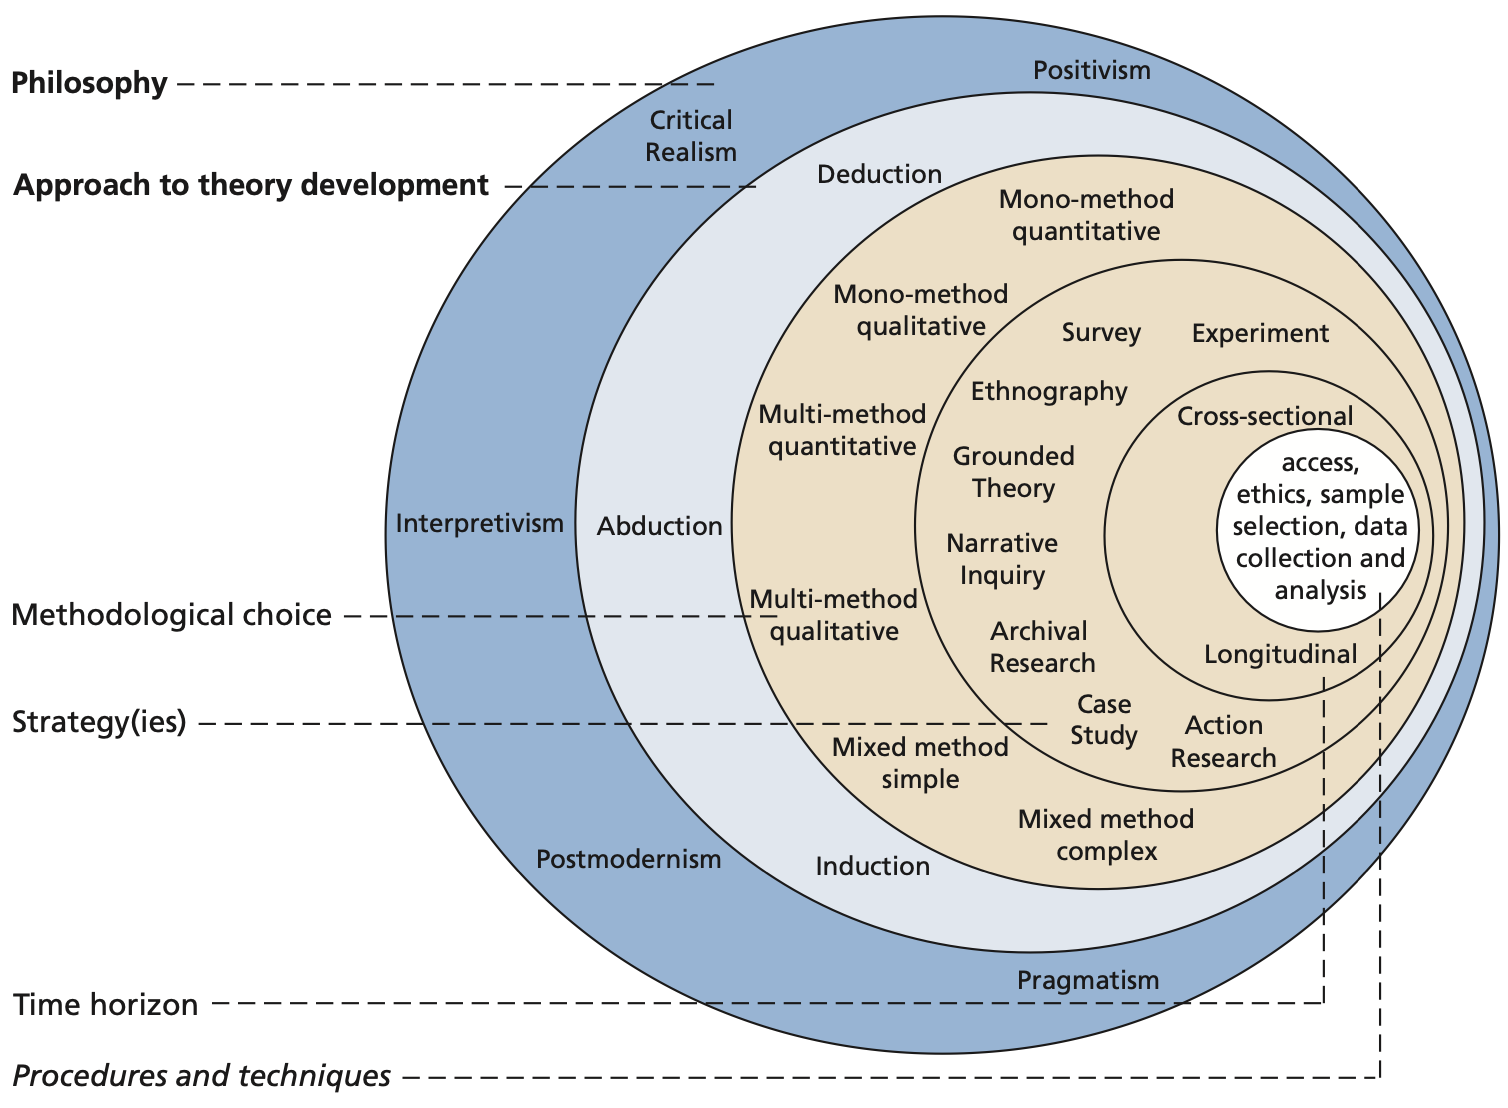
\includegraphics[width=.9\textwidth]{figures/research-design/research-onion.png}
     \rule{35em}{0.5pt}
    \caption{The Research onion (\textcite{SaundersMark2023})} 
 \label{fig:research-onion}
\end{figure}

\section{Research Philosophy}\label{sec:research-philosophy}
Research philosophy is the first layer of the research onion and refers to the set of beliefs and assumptions that establish the research process.
Following the research onion \cite{SaundersMark2023}, the main philosophies that a researcher can adopt are positivism, critical realism, interpretivism, postmodernism, and pragmatism.

\textit{Positivism} is based on the idea of working with an observable social reality and that the end product of such research can be generalisations similar to those produced by physical and natural scientists.
Since it argues for an objective reality that can be measured by quantitative methods, this thesis does not follow this approach as the main objective is not to generalise the findings.
\textit{Critical realism} is based on the idea that the social world is not a direct reflection of the physical world, but that it is constructed by individuals based on their experiences and perceptions.
This approach is also not followed in this study as it is more focused on understanding the social world as it is perceived by the participants.
\textit{Interpretivism} emphasizes the importance of understanding the differences among human beings in their roles as social actors.
It highlights the distinction between conducting research involving people, who interpret and assign meaning to their experiences, as opposed to research involving inanimate objects.
This thesis does not follow this philosophy because it does not explore subjective human experiences and social constructs.
\textit{Postmodernism} challenges established ideas by emphasizing the role of language, power, and cultural context in shaping reality.
It rejects the notion of a single objective truth, arguing instead for multiple, evolving perspectives influenced by social constructs.
This philosophy is not followed in this thesis as it does not aim to challenge established ideas or explore the role of language, power, and cultural context in shaping reality.
Finally, \textit{pragmatism} focuses on practical solutions, asserting that research should be guided by the problem at hand rather than rigid philosophical stances.
It promotes flexibility by combining qualitative and quantitative methods to achieve useful and actionable outcomes.

This thesis follows a pragmatic approach in that it aims to address the problem of finding collaborators for a given research project.
%
\section{Research Approach}\label{sec:research-approach}
According to \textcite{SaundersMark2023}, the second layer of the research onion is the research approach, which is the strategy that the researcher can use to start the research.
There are three main research approaches.
\textit{Deductive} approach, that begins with established theories or hypotheses and tests them through empirical data collection, following a structured and logical progression to confirm or refute existing concepts.
In contrast, \textit{inductive} approach involves deriving theories from observed data, allowing patterns and relationships to emerge without predefined expectations.
\textit{Abductive} approach combines elements of both, iteratively moving between theory and data to refine explanations and generate new insights based on surprising observations.

This thesis follows the inductive approach because the aim is to design and develop a system that is based on a data domain, the European research domain.
The data collection to provide this recommendation of collaborators starts with the research questions for analysis, experiments and evaluation of a prototype.
This prototype will be based on a hybrid \gls{ai} approach, the performance of which will be measured by certain evaluation metrics.
The results obtained will be used to prove the thesis statement.
%
\section{Methodological Choice}\label{sec:methodological-choice}
The third layer of the research onion is the methodological choice, which refers to the specific techniques and procedures used to collect and analyze data.
According to \textcite{SaundersMark2023}, the methodological choice is influenced by the research philosophy and approach.

Research can be conducted using either a quantitative or qualitative approach, depending on the objectives pursued.
Quantitative research is primarily concerned with hypothesis testing through a deductive approach or pattern discovery when adopting an inductive perspective.
In both cases, the analysis relies on a large volume of data to ensure statistical significance.
In contrast, qualitative research focuses on smaller datasets, aiming to capture the underlying characteristics within them.

This thesis use a qualitative research approach, as the primary goal is to understand the research domain and the challenges faced by researchers in finding collaborators.
%
\section{Research Strategy}\label{sec:research-strategy}
The research strategy defines how the research goal is to be achieved \cite{SaundersMark2023}.
This aspect of the research design is crucial as it outlines the steps to be taken to address the research questions effectively.
Several research strategies have been defined including: Experiment, Survey, Case study, Action research, Grounded theory, Ethnography and Archival research.
Each of these strategies is designed with a specific purpose in mind and is best suited to achieving the intended research objective.

Since the primary goal of this thesis is to design and develop an artefact, the research strategy used is the \gls{dsr} \cite{Hevner2010}.
\gls{dsr} is a research methodology that focuses on what is called ``relevance'', which is the creation and evaluation of an artifact to solve complex real-world problems.
Moreover, the research should enhance the existing body of knowledge, a principle referred to as ``rigor''.
This duality emerges from the fundamental idea that \gls{dsr} combines two distinct research paradigms: behavioral science and design science, each serving unique objectives to achieve the overall research goals.
A proposed Information Systems Research framework (Fig.~\ref{fig:information-system-research-framework}) illustrates this dual nature, emphasizing the necessity of addressing both a practical business need and the application of relevant knowledge in the research process.

\begin{figure}[htbp]
    \centering
 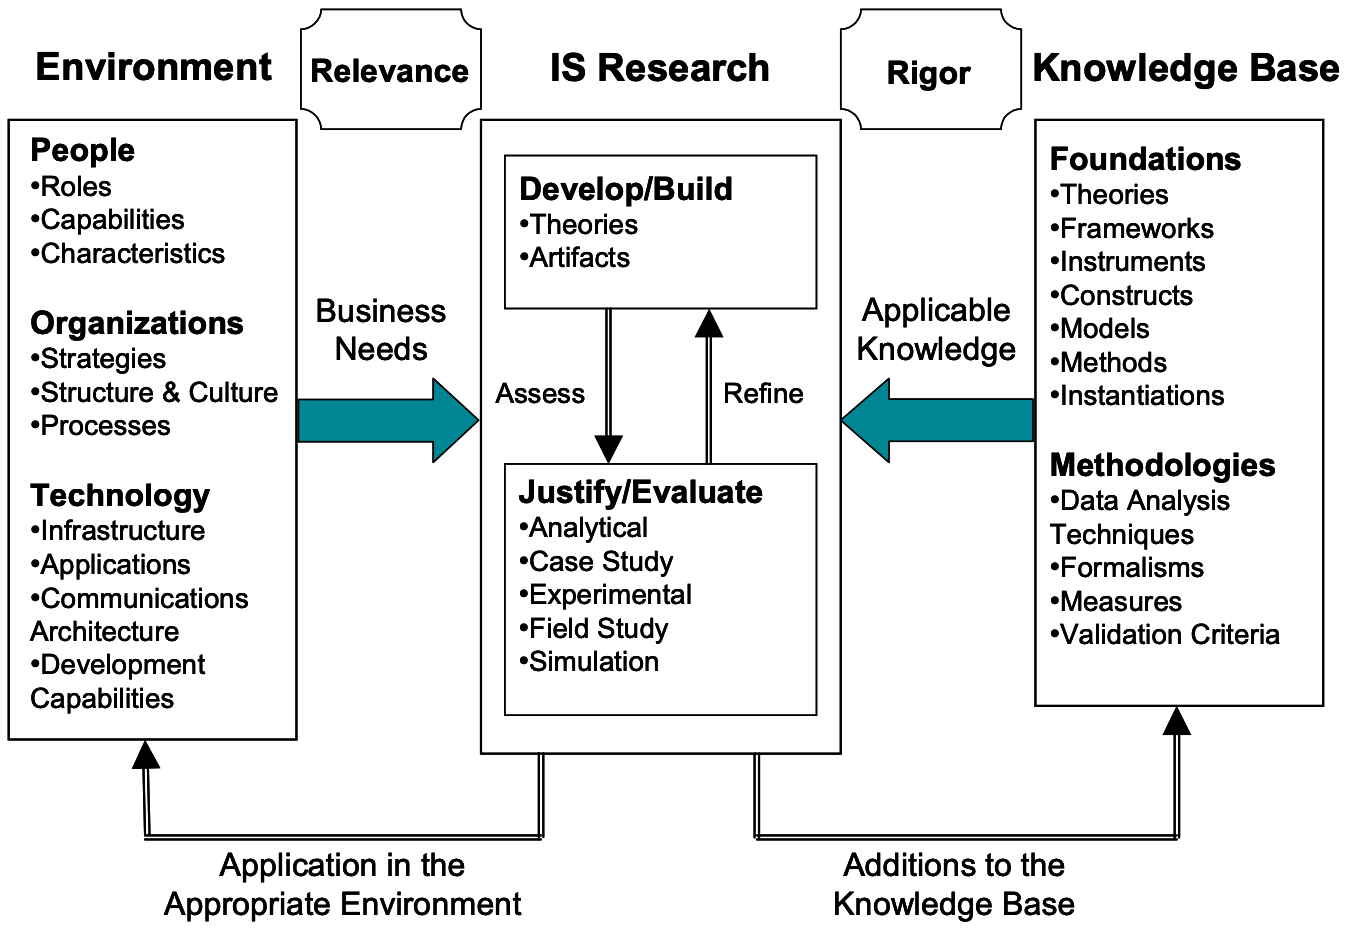
\includegraphics[width=.9\textwidth]{figures/research-design/information-system-research-framework.png}
     \rule{35em}{0.5pt}
    \caption{Information Systems Research Framework (\textcite{Hevner2010})} 
 \label{fig:information-system-research-framework}
\end{figure}

As already mentioned, the \gls{dsr} focuses on the creation and evaluation of an artifact to solve complex real-world problems.
The \gls{dsr} process is iterative, involving multiple cycles of development and evaluation, as illustrated in Fig.~\ref{fig:design-science-research-cycles}.

\begin{figure}[htbp]
    \centering
 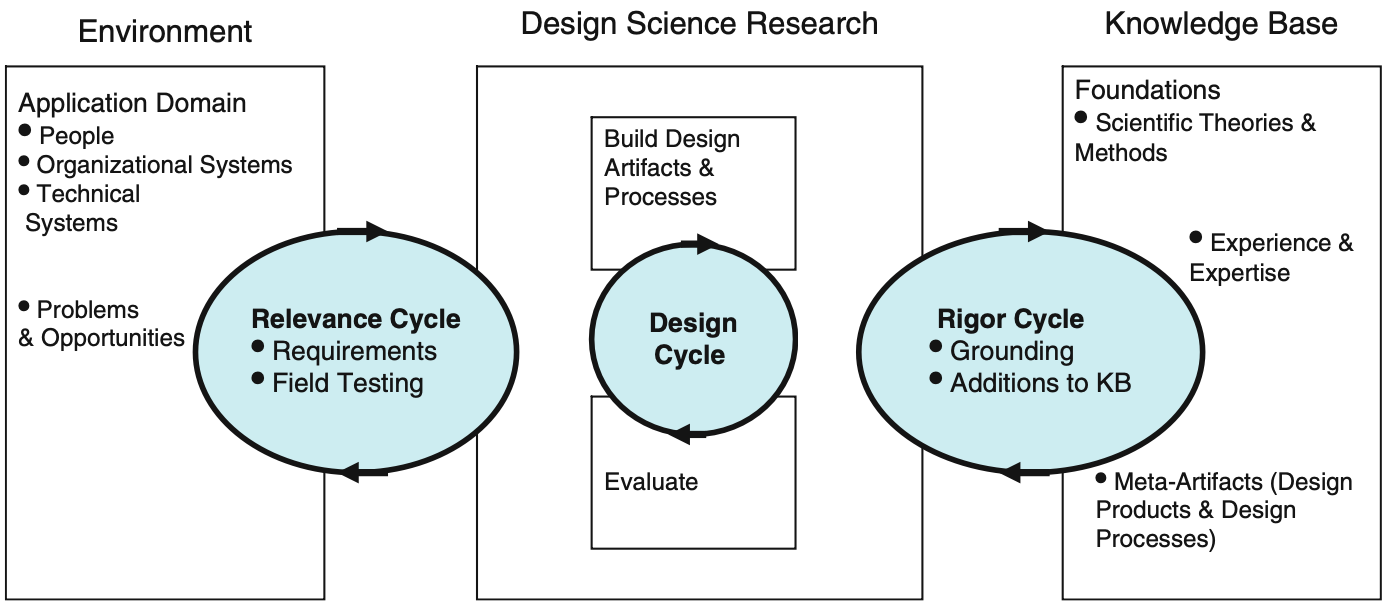
\includegraphics[width=.9\textwidth]{figures/research-design/design-science-research-cycles.png}
     \rule{35em}{0.5pt}
    \caption{\acrlong{dsr} Cycles (\textcite{Hevner2010}) } 
 \label{fig:design-science-research-cycles}
\end{figure}

On the right side, the Rigor Cycle focuses on existing knowledge, incorporating theories, methodologies, and expert experiences.
In the context of this thesis, it represents the literature review.
On the left side, the Relevance Cycle highlights the application domain, encompassing the people, organizations, systems, and the challenges or opportunities they face.
At the center, there is the Design Cycle, which addresses research through the development and evaluation of the artifact.
These three components are interconnected, forming a continuous \gls{dsr} cycle that ensures the integration of knowledge, practical relevance, and iterative refinement.

According to \textcite{Hevner2010}, the \gls{dsr} is defined in five process steps: awareness of problem, suggestion, development, evaluation, and conclusion.
\textcite{Hevner2010} modified a framework originally proposed by \textcite{Vaishnavi2007}, illustrating the five process steps along with the expected outputs and knowledge flows, as illustrated in Fig.~\ref{fig:design-science-research-framework}.

\begin{figure}[htbp]
    \centering
 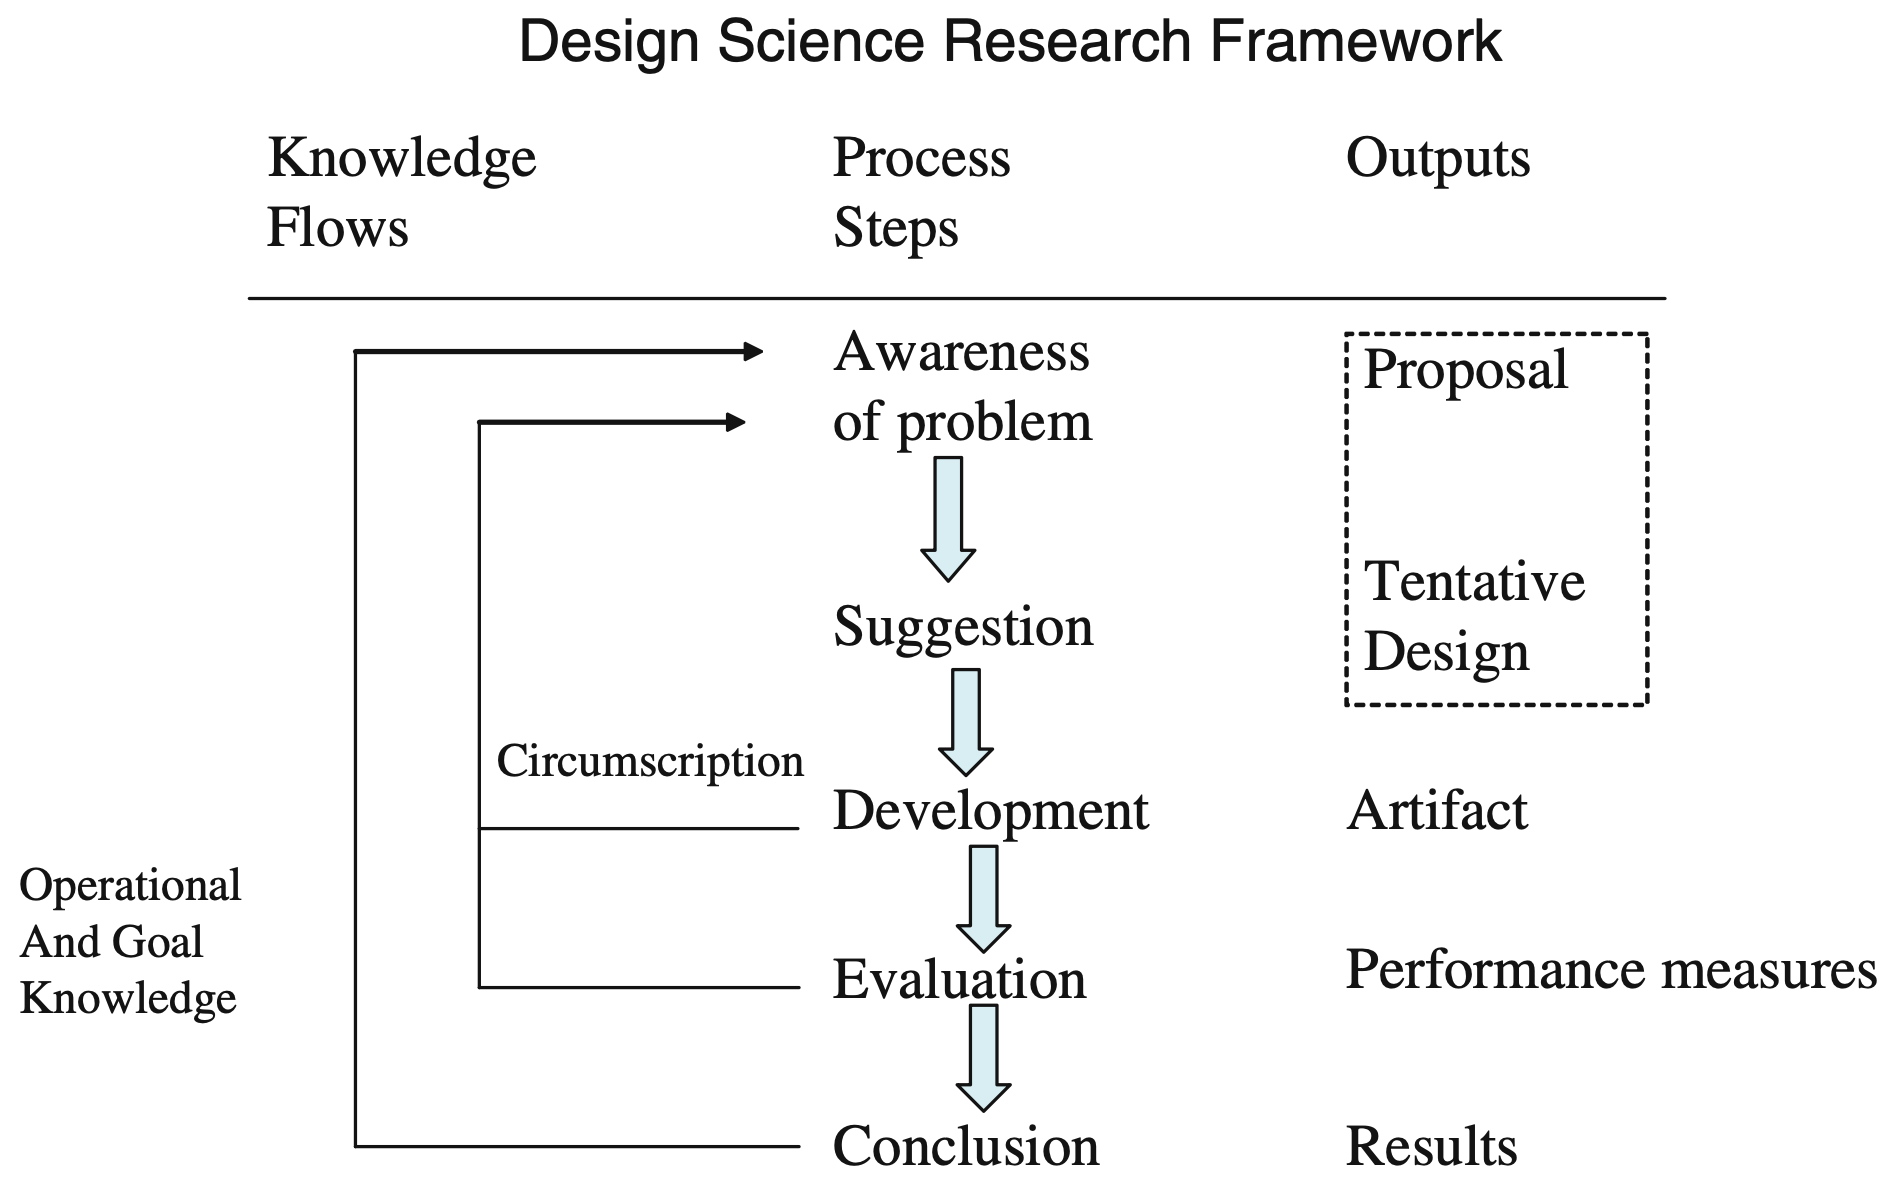
\includegraphics[width=.9\textwidth]{figures/research-design/design-science-research-framework.png}
     \rule{35em}{0.5pt}
    \caption{\acrlong{dsr} Framework (\textcite{Hevner2010}) adapted from (\textcite{Vaishnavi2007})} 
 \label{fig:design-science-research-framework}
\end{figure}

The research of this thesis will follow the \gls{dsr} methodology, in accordance with the five steps of the framework proposed by \textcite{Hevner2010}.

The Awareness Phase involves researchers identifying and recognizing a specific problem or opportunity that requires attention.
During this initial stage, they gain a clear understanding of existing challenges or gaps in current systems or processes, laying the groundwork for the subsequent phases of the design cycle.

In the Suggestion Phase, researchers propose potential solutions to address the identified problem or opportunity.
This stage focuses on generating innovative ideas and design concepts that serve as the foundation for developing artifacts aimed at resolving the issue.

The Development Phase is where researchers build and implement the designed artifacts or solutions based on the proposals from previous phases.
This stage transforms conceptual designs into functional prototypes, bringing the ideas to life.

During the Evaluation Phase of \gls{dsr}, researchers analyze and assess the developed artifacts to determine their effectiveness and performance.
This stage involves rigorous testing, validation, and evaluation of the solutions against predefined criteria and objectives.
Stakeholder feedback may also be collected to refine and enhance the artifacts further.
The primary goal of this phase is to ensure that the designed solutions effectively address the identified problem and meet the intended requirements.

Finally, the Conclusion Phase involves drawing insights and summarizing findings based on the outcomes of the evaluation phase.
Researchers reflect on the effectiveness of the designed artifacts, assess their impact on solving the identified problem, and evaluate their overall contribution to the research objectives.

Fig.~\ref{fig:design-science-research-framework-adapted-by-author} illustrates the \gls{dsr} framework adapted by the author, which will be used to guide the research process in this thesis.
Each of these \gls{dsr} steps applied to this thesis is mapped and described in the following chapters.
\begin{figure}[htbp]
    \centering
 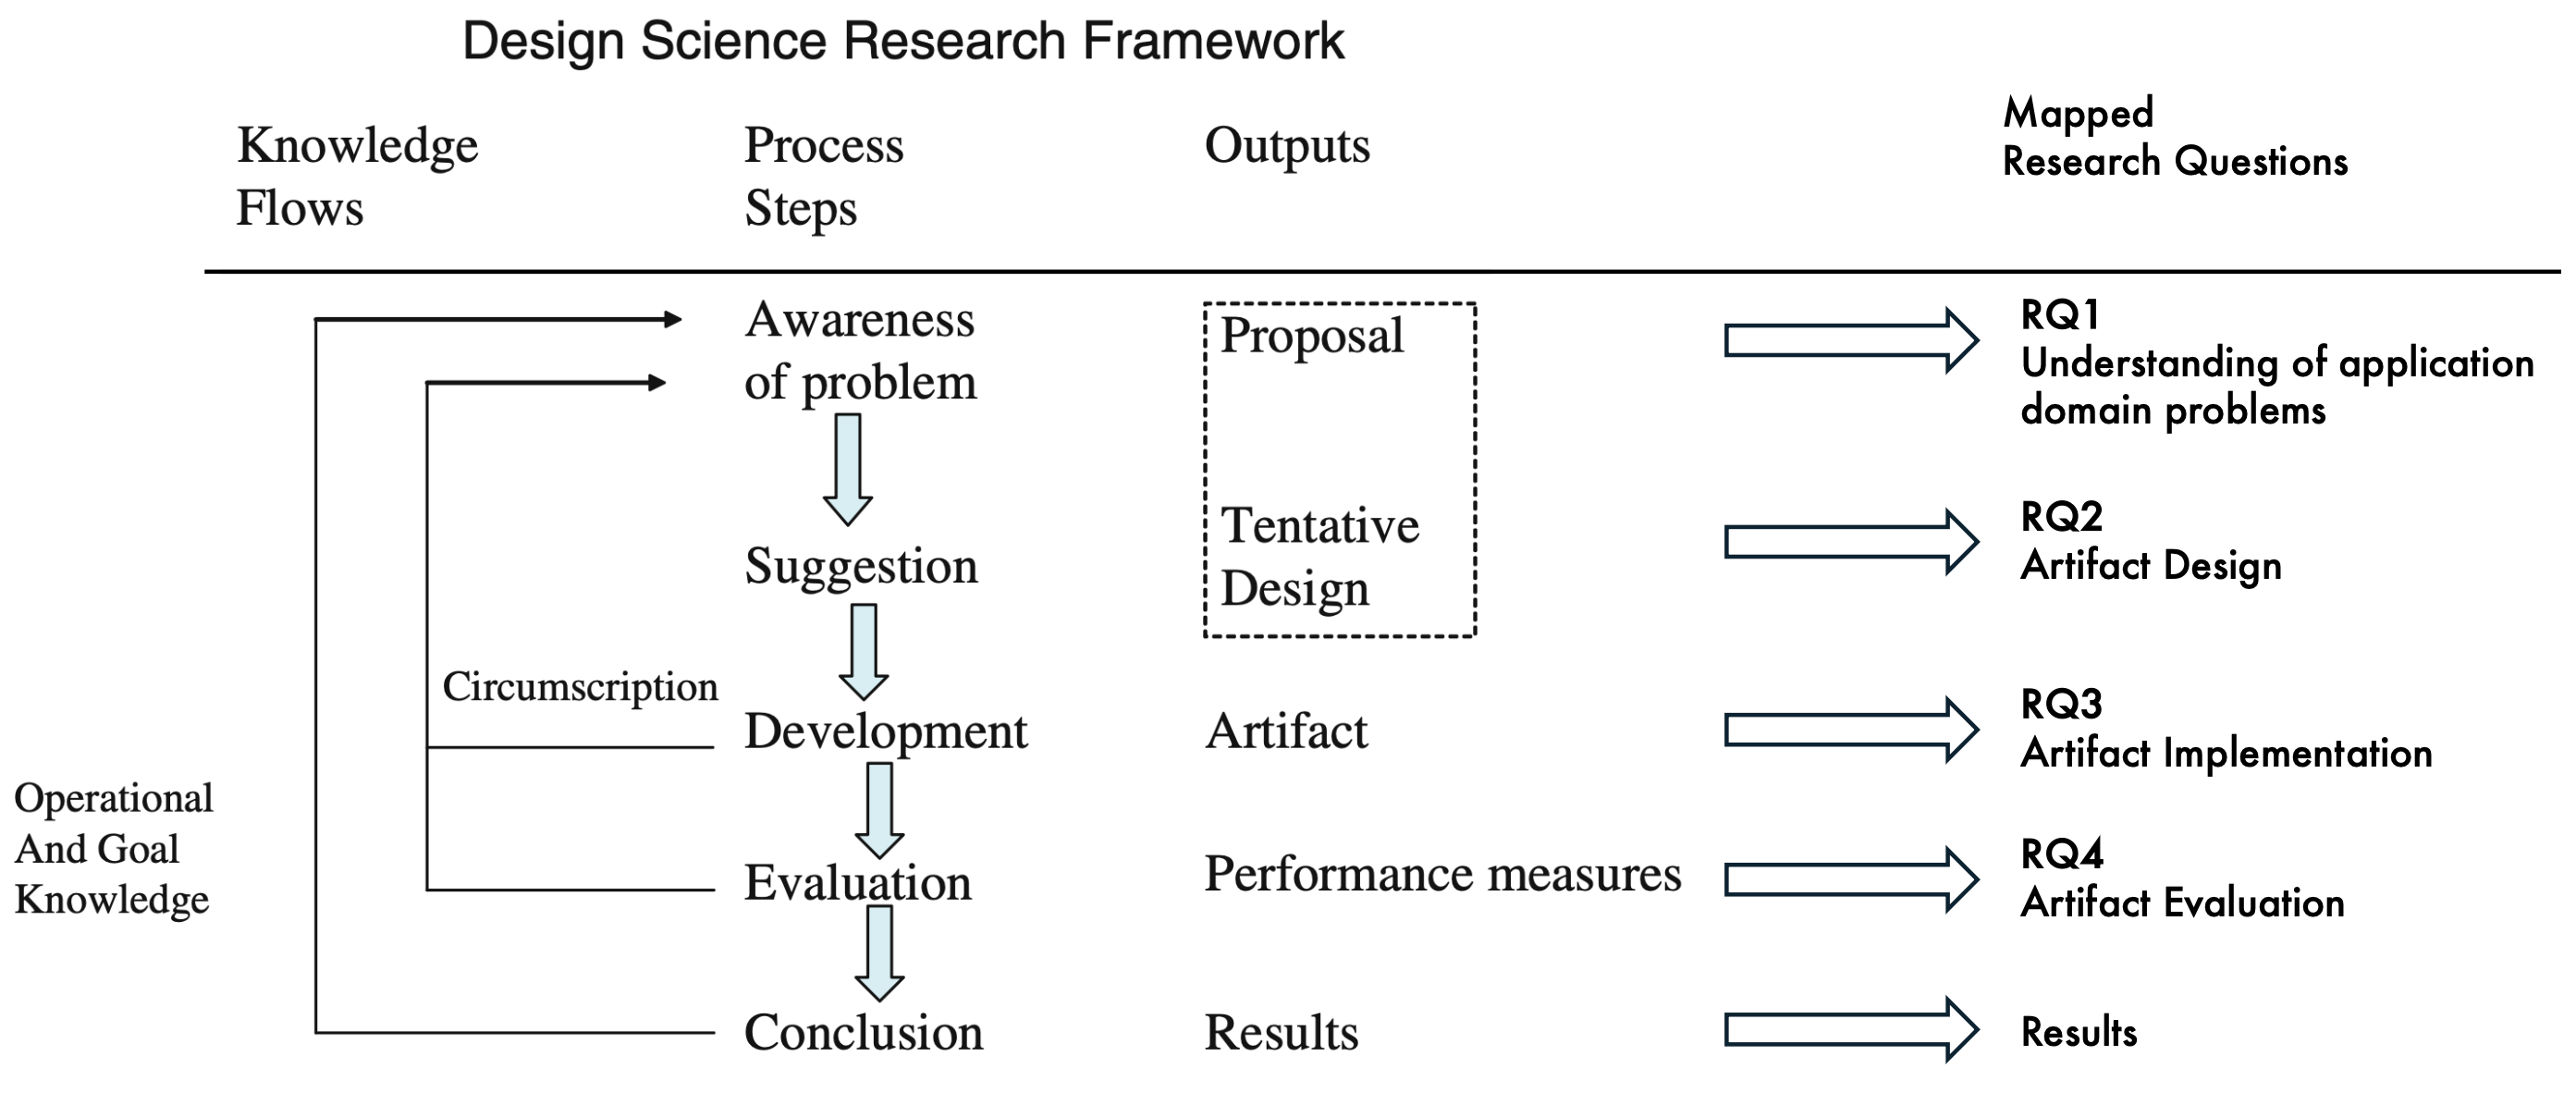
\includegraphics[width=.9\textwidth]{figures/research-design/design-science-research-framework-by-author.png}
     \rule{35em}{0.5pt}
    \caption{\acrlong{dsr} Framework adapted by the author} 
 \label{fig:design-science-research-framework-adapted-by-author}
\end{figure}


%
\section{Time Horizon}\label{sec:time-horizon}
This layer of the research onion focuses on the research's time horizon, distinguishing between longitudinal and cross-sectional approaches \cite{SaundersMark2023}.
Longitudinal research extends over an extended period, capturing multiple snapshots throughout the study.
In contrast, a cross-sectional approach examines a single snapshot within a specific, typically shorter, timeframe.
Given time constraints, this thesis adopts a cross-sectional time horizon, namely the duration of the thesis development.
%
\section{Data Collection and Data Analysis}\label{sec:data-collectiom-and-data-analysis}
Data collection is the systematic process of gathering and measuring information on specific variables to answer relevant questions and assess outcomes.
According to \textcite{SaundersMark2023}, there are four primary methods of data collection:
\begin{itemize}
    \item Questionnaires: these are an efficient way to collect data as they consist of fixed-response questions that can be easily analyzed and compared. However, a key limitation is that participants cannot clarify their answers, which may lead to misinterpretations.
    \item Interviews: interviews can be structured like questionnaires, semi-structured with a mix of predefined and open-ended questions, or unstructured, allowing the interviewer to guide the conversation. While interviews are typically conducted one-on-one, they can also be held in group settings. A major challenge is finding suitable interview participants, and there is always a risk of bias. Additionally, conducting multiple interviews can be time-consuming.
    \item Observation: in observational research, a researcher studies participants' behavior to identify patterns. While this method provides real-world insights, interpreting observations correctly and selecting appropriate subjects for observation can be challenging.
    \item Archival Research: this method involves analyzing historical documents and textual materials from organizations or institutions. It provides valuable insights from past data but may require extensive interpretation and verification.
\end{itemize}

Data analysis refers to the process that takes place after data collection, aiming to extract meaningful insights and patterns from the gathered information.

In this thesis, no questionnaires, interviews, observations, or archival research methods were employed, as the focus was strictly on the European research domain.
Given that the dataset used, detailed in the next chapter (Sec.~\ref{sec:dataset}), specifically pertains to EU-funded research projects, the analysis was conducted solely within this structured data framework, ensuring relevance to the scope of European research.